\section{Evaluation}
%在本章节中,我们主要从以下几个角度进行评估:1)规则冲突的检测的有效性;2)自动化规则冲突解决的可用性;3)系统的性能。
In this chapter, we mainly evaluate from the following perspectives: 1) The effectiveness of static detection of rule conflicts; 2) The viability of automated conflict resolution; 3) The performance of the system.

\begin{figure}[htbp]
	\centering
	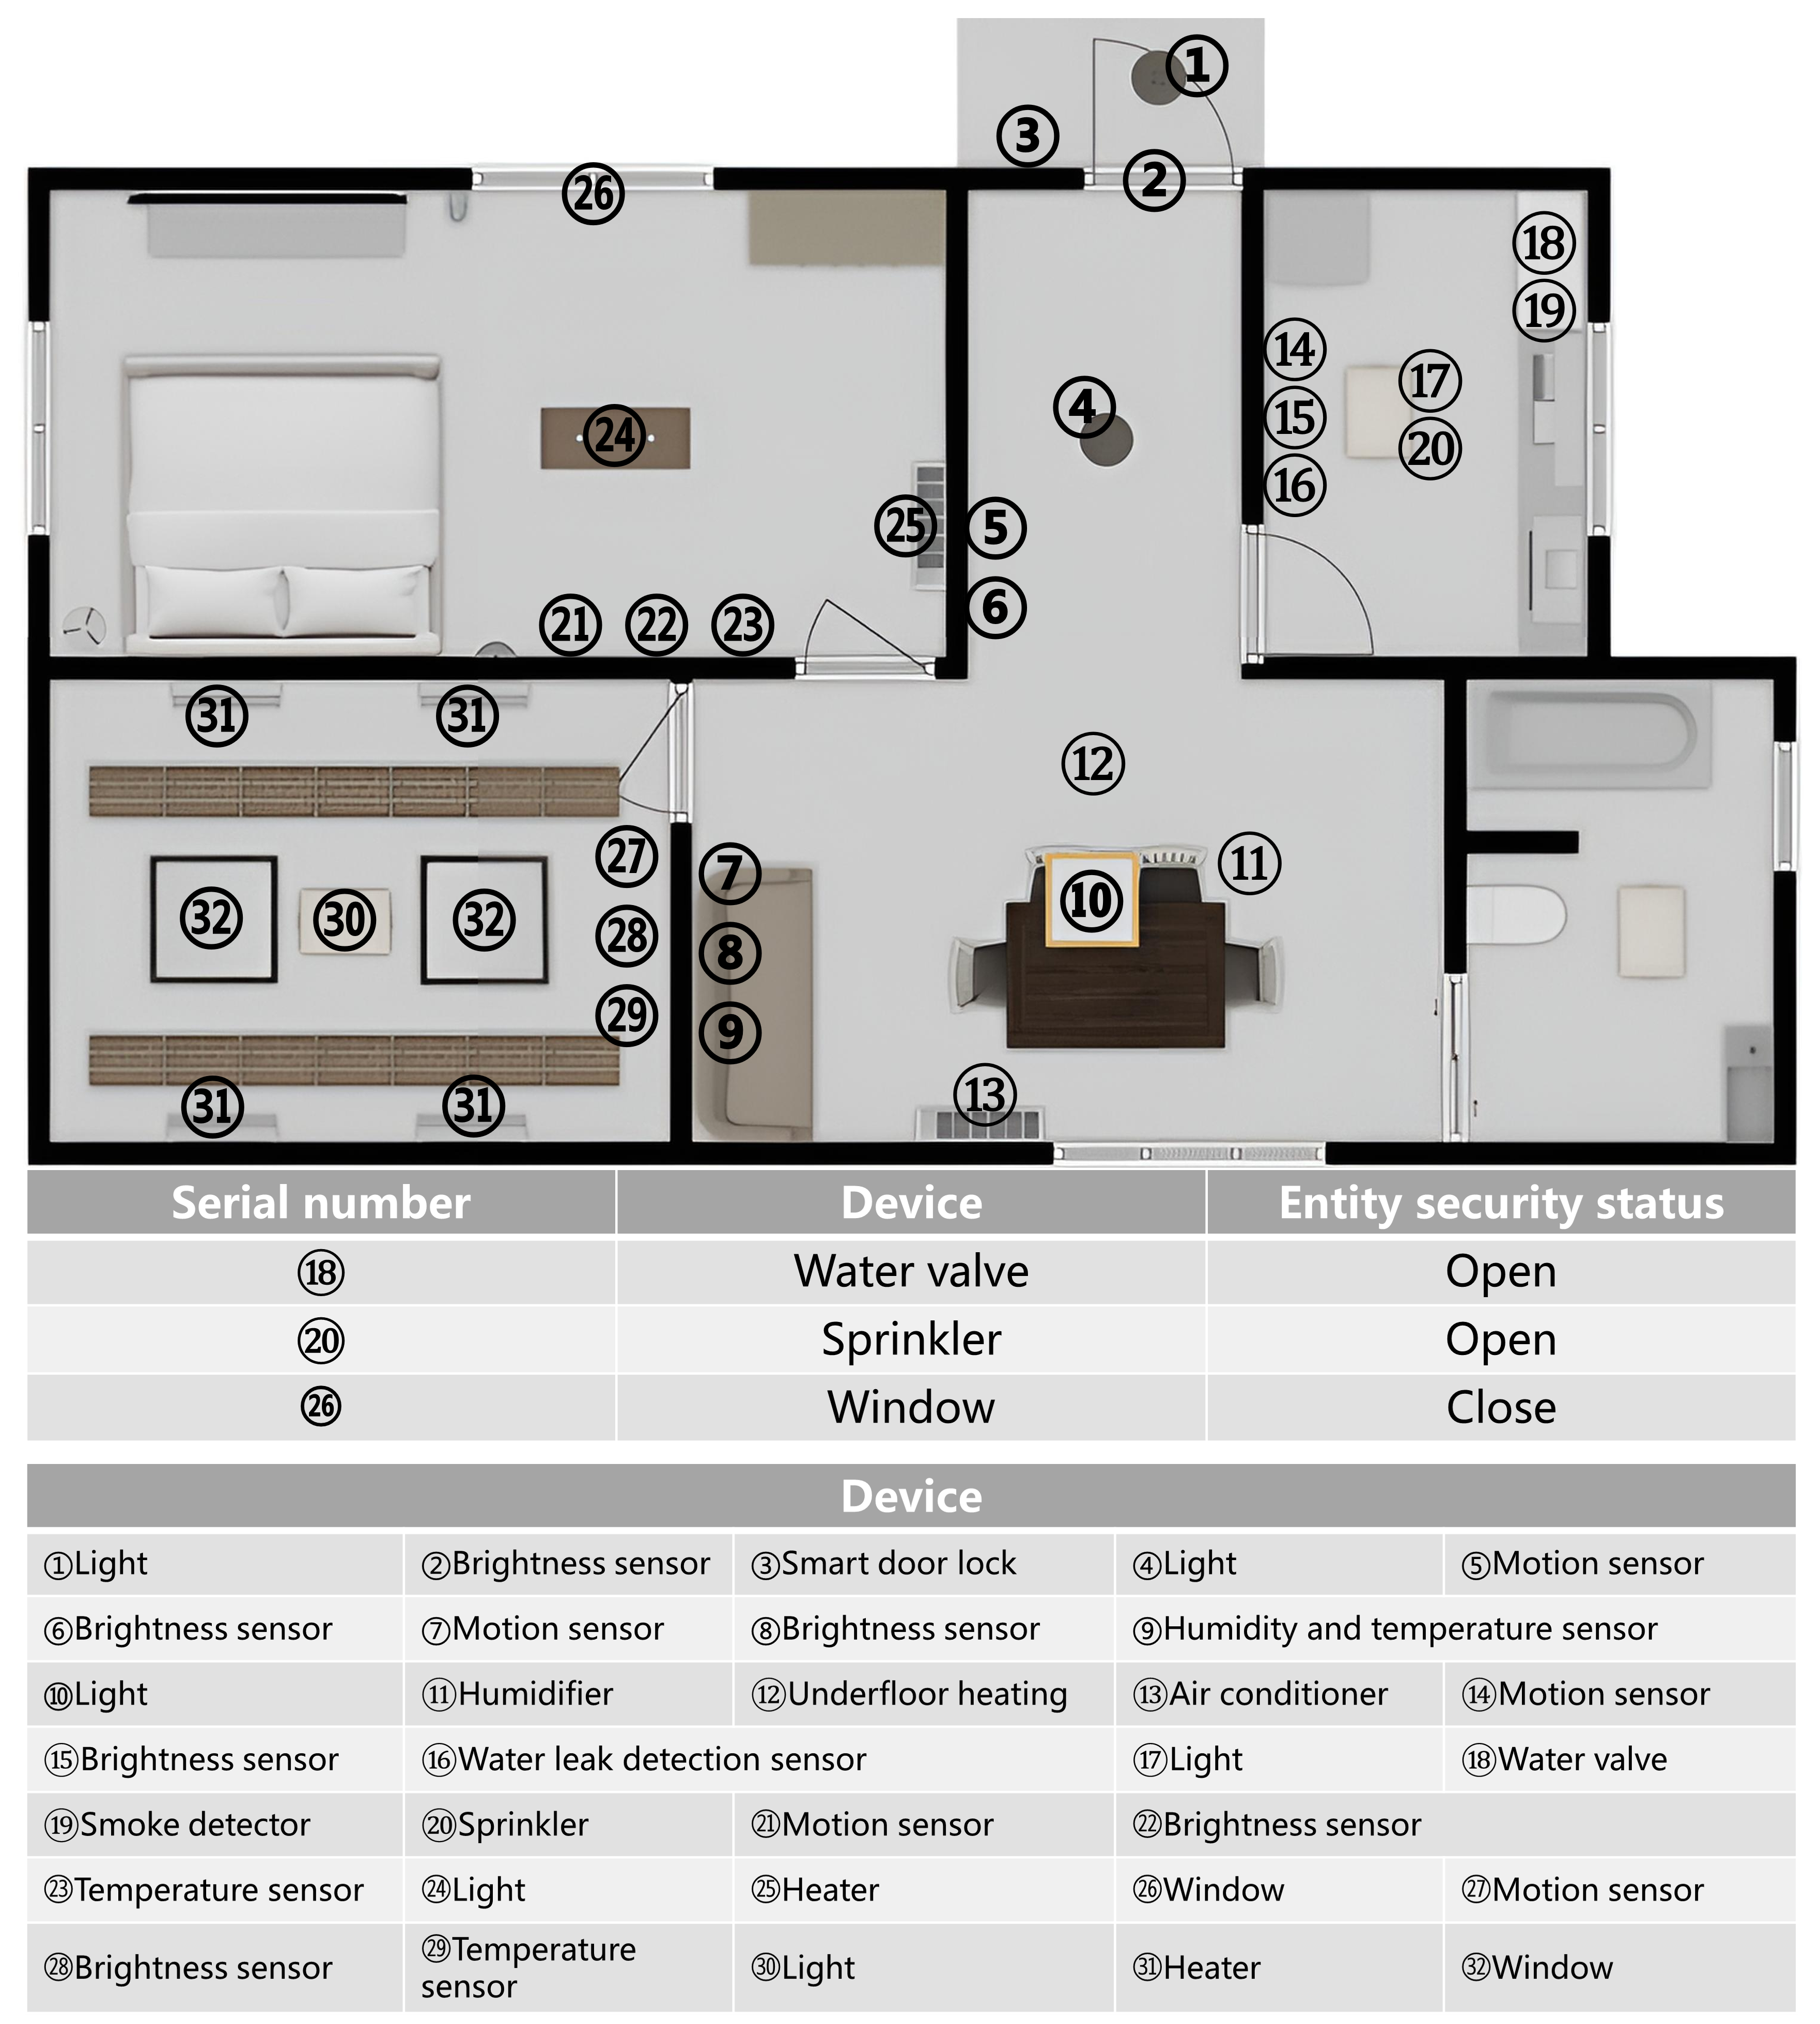
\includegraphics[width=0.5\textwidth]{figure/smarthome.png}
	\caption{Smart Home Floor Plan}
	\label{smarthome_floorplan}
\end{figure}

\subsection{Smart Home Testbeds}

%我们实现了一个完整的系统并进行了虚拟测试。对于虚拟测试,选择了基于 Python 的开源智能家居平台 Home Assistant。Home Assistant 支持来自各种制造商的设备,并提供虚拟设备以实现自动化功能。在此平台上,用户可以通过可视化 Web 界面或直接编辑配置文件来定义自定义自动化规则。Home Assistant 使用 YAML 配置文件来描述自动化规则,采用触发-条件-动作 (TCA) 模型。
We implements a complete system and conducts a virtual test. For the virtual test, Home Assistant, an open-source smart home platform based on Python, was selected.Home Assistant supports devices from various manufacturers and provides virtual devices to enable automation functionalities. On this platform, users can define custom automation rules either through a visual web interface or by directly editing configuration files. Home Assistant uses YAML configuration files to describe automation rules, employing a trigger-condition-action (TCA) model.

%虚拟测试使用图 \ref{smarthome_floorplan} 中所示的智能家居平面图。模拟的智能家居环境由七个不同的区域组成:室外、门廊、客厅、厨房、浴室、卧室和温室(花园)。根据观察,特定区域中的某些通道会相互影响。例如,门廊和客厅的亮度属性是相互依赖的,而客厅和卧室的亮度属性是独立的。
The virtual test uses the smart home floor plan illustrated in Figure \ref{smarthome_floorplan}. The simulated smart home environment consists of seven distinct zones: Outdoor, Porch, Living Room, Kitchen, Bathroom, Bedroom, and Greenhouse (Garden).  Based on observations, certain channels in specific zones can influence each other. For instance, the brightness attributes of the porch and living room are interdependent, while the brightness attributes of the living room and bedroom are independent.

%表 \ref{Testbeds} 列出了在这七个区域配置的 17 个自动化规则,以及相应的区域和设备。表 \ref{side_channel} 详细说明了智能家居系统中配置的侧通道,其中每个侧通道由一个区域、一个通道和一个趋势定义。最后,Figure.\ref{smarthome_floorplan} 概述了智能家居系统中的实体安全配置,特别关注三个安全敏感设备的状态设置:水阀(开启)、喷水灭火器(开启)和卧室窗户(关闭)。
Table \ref{Testbeds} lists the 17 automation rules configured across these seven zones, along with the corresponding zones and devices. Table \ref{side_channel} details the side channels configured within the smart home system, where each side channel is defined by a zone, a channel, and a trend. Finally, Figure.\ref{smarthome_floorplan} outlines the entity security configurations in the smart home system, specifically focusing on the state settings for three security-sensitive devices: water valve (On), sprinkler (On), and bedroom window (Closed).

\begin{table}[htbp]
	\caption{Classification of Side Channel Attributes Across Different Home Zones}
	\label{side_channel}
	\begin{tabular}[width=0.45\textwidth]{l|l|l}
		\hline
		\textbf{Zone} & \textbf{Channel} & \textbf{Trend} \\
		\hline
		outdoor& brightness, & increase/decrease \\
		\hline
		porch& brightness, & increase/decrease \\
		\hline
		kitchen& brightness,temperature & increase/decrease \\
		\hline
		living room & brightness,humidity,temperature & increase/decrease \\
		\hline
		bedroom & brightness,temperature & increase/decrease \\
		\hline
		greenhouse & brightness,temperature & increase/decrease \\
		\hline
	\end{tabular}
\end{table}


\begin{table*}[htbp]
	\caption{Testbed: Details of Experimental Smart Home Rules (R1-R17)}
	\label{Testbeds}
	\centering
	\begin{adjustbox}{width=\textwidth}
	\begin{tabular}{c|l|c|l}
		\hline
		\textbf{Rule ID} & \textbf{Content} & \textbf{Area} & \textbf{Devices} \\
		\hline
		R1 & When the door lock is opened, if the brightness sensor is below 50lux, turn on the outdoor light and porch light. & Outdoor & \circled{1} \circled{2} \circled{3} \circled{4} \\
		\hline
		R2 & When the door lock is closed, turn off the porch light. & Outdoor & \circled{3} \circled{4} \\
		\hline
		R3 & When motion is detected in the porch, if the brightness sensor is below 50lux, turn on the porch light. & Porch & \circled{4} \circled{5} \circled{6} \\
		\hline
		R4 & When motion is detected in the living room, if the brightness sensor is below 50lux, turn on the living room light. & Living Room & \circled{7} \circled{8} \circled{10}\\
		\hline
		R5 & When the living room humidity is below 40\%, and the humidifier is off, turn on the living room humidifier. & Living Room & \circled{9} \circled{11} \\
		\hline
		R6 & When the living room humidity is above 60\%, turn off the living room humidifier. & Living Room & \circled{9} \circled{11} \\
		\hline
		R7 & When the living room temperature is below 24°C, turn off the living room floor heating and turn on the underfloor heating. & Living Room & \circled{9} \circled{12}\\
		\hline
		R8 & When the living room temperature is above 30°C, turn off the living room air conditioner and set it to 27°C. & Living Room & \circled{9} \circled{13} \\
		\hline
		R9 & When motion is detected in the kitchen, if the brightness sensor is below 50lux, turn on the kitchen light. & Kitchen & \circled{14} \circled{15} \circled{17} \\
		\hline
		R10 & When a water leak is detected, close the main water valve. & Kitchen & \circled{16} \circled{18} \\
		\hline
		R11 & When the smoke detector is triggered, turn on the sprinkler. & Kitchen & \circled{19} \circled{20} \\
		\hline
		R12 & When motion is detected in the bedroom, if the brightness sensor is below 50lux, turn on the bedroom light. & Bedroom & \circled{21} \circled{22} \circled{24} \\
		\hline
		R13 & At 7 PM, turn on the bedroom heating. & Bedroom & \circled{25} \\
		\hline
		R14 & When the bedroom temperature reaches 30°C, open the window and close the heating. & Bedroom & \circled{23} \circled{25} \circled{26} \\
		\hline
		R15 & When motion is detected in the green house, if the brightness sensor is below 50lux, turn on the green house light. & Green house & \circled{27} \circled{28} \circled{30}\\
		\hline
		R16 & At 7 PM, turn on the green house heating. & Green house & \circled{31} \\
		\hline
		R17 & When the green house temperature reaches 32°C, open the window and close the heating. & Green house & \circled{29} \circled{31} \circled{32} \\
		\hline
	\end{tabular}
	\end{adjustbox}
\end{table*}

\subsection{Effectiveness of Conflict Detection}
%为了评估规则冲突的检测有效性,采用手动触发的方式测试所有可能的规则交互,并手动检测出其中存在的四条规则冲突,每条规则冲突可能对应多种规则冲突类型,然后使用本论文实现的系统进行静态检测与动态检测(同样采用手动触发的方式),同时对比了IoTMEDIATOR的检测结果。
In order to evaluate the effectiveness of rule conflict detection, all possible rule interactions were tested using manual triggering, and four rule conflicts were identified(Each rule conflict can correspond to multiple rule conflict types). Subsequently, the system implemented in this paper was used for both static and dynamic detection (also through manual triggering), while also comparing the detection results with those of IoTMEDIATOR.

%所有七个区域的17条规则的冲突测试结果如Table.\ref{conflict_detection_result}所示,其中R10-R11存在规则冲突:R10会控制水阀关闭,导致在R11被触发时,R11无法正常执行。R11-R10存在规则冲突:R11执行时,会触发R10的执行,且R11的执行动作与R10的执行动作互斥。R13-R14存在规则冲突:R13的执行会触发R14的执行,且两条规则的执行动作互斥。R14-R13存在规则冲突:R14的执行结果与R13的执行结果互斥。
The conflict results of 17 rules in all seven regions are shown in Table.\ref{conflict_detection_result}. Among them, there is a conflict between R10 and R11: R10 controls the water valve to close, causing R11 to fail execution when triggered. There is also a conflict between R11 and R10: when R11 is executed, it triggers the execution of R10, and the execution actions of R11 and R10 are mutually exclusive. Additionally, there is a conflict between R13 and R14: the execution of R13 triggers the execution of R14, and the execution actions of both rules are mutually exclusive. There is also a conflict between R14 and R13: the execution result of R14 is mutually exclusive with that of R13.

%测试结果表示IoTMEDIATOR能够检测到其中的R11-R10、R13与R14与R14-R13的规则冲突,而无法检测到R10与R11通过humidity的side channel互相影响导致的规则冲突,即智能家居系统检测到漏水后关闭水阀,此后如果用户没有及时处理,如果引发火灾,水阀仍旧没有开启,R11无法正常执行。同时IoTMEDIATOR坚持到了许多其他的规则交互,但是他们是否属于规则冲突需要用户进行根据主观偏好进行选择。例如:规则 R5 控制客厅加湿器以增加湿度,而规则 R6 控制加湿器以关闭以防止湿度过高。这两条规则之间的交互能够便捷地维持客厅湿度,不应被视为规则冲突。(IoTMEDIATOR对于Race Condition、 Potential Race Condition和Condition Bypass时对称的,即两条规则对应两次规则冲突,在表格中可能只展示一次,后续需要修改——zyd)
The test results indicate that IoTMEDIATOR is able to detect the rule conflicts of R11-R10, R13 with R14, and R14-R13, but it fails to detect the rule conflict caused by the mutual influence through humidity between R10 and R11. Specifically, after the smart home system shuts off the water valve upon detecting a water leak, if the user does not respond in time and a fire is triggered, the water valve will not open, resulting in R11 not executing normally. Meanwhile, IoTMEDIATOR persists with many other rule interactions; however, whether they constitute rule conflicts is subject to the user's subjective preference. For example, R5 controls the living room humidifier to increase humidity, while R6 controls the humidifier to shut off in order to prevent excessive humidity. The interaction between these two rules conveniently maintains the living room’s humidity and should not be regarded as a conflict.

%所有规则交互都能被我们的系统精确捕捉,同时能够自动将任何威胁性规则交互是为规则冲突,从而检测到所有的四条规则冲突,并检测出六种可能的冲突发生方式。除此之外,我们的系统能够有效避免规则冲突的误报,极大程度上避免了将正常的规则交互错误分类到规则冲突的可能性,与此同时用户可以将其他规则交互根据个人偏好选择是否列入规则冲突列表中。
All rule interactions can be precisely captured by our system, and it is capable of automatically converting any threatening rule interactions into rule conflicts, thereby detecting all four types of rule conflicts and identifying six possible ways in which conflicts might occur. In addition, our system effectively avoids false positives in identifying rule conflicts, greatly minimizing the chance that normal rule interactions are mistakenly classified as conflicts, while also allowing users to optionally include other rule interactions in the rule conflict list according to their personal preference.

%\begin{table*}[htbp]
%	\centering
%	\caption{Result of Rule Conflict Detection}
%	\label{conflict_detection_result}
%	\begin{adjustbox}{width=\textwidth}
%		\begin{tabular}{|c|l|c|c|c|c|c|c|c|c|c|c|c|c|c|} 
%			\hline
%			& \textbf{Classification} & \textbf{R1-R2} & \textbf{R2-R1} & \textbf{R2-R3} & \textbf{R3-R2} & \textbf{R5-R6} & \textbf{R6-R5} & \textbf{R9-R3} & \textbf{R10-R11} & \textbf{R11-R10} & \textbf{R13-R14} & \textbf{R14-R13} & \textbf{R15-R12} & \textbf{R16-R17} \\ \hline
%			\multirow{6}{*}{\rotatebox{90}{Ours}} & Rule Trigger Conflict &  &  &  &  &  &  &  &  &  &  &  &  &  \\
%			\cline{2-15}
%			& Rule Condition Conflict &  &  &  &  &  &  &  &  &  &  &  &  &  \\
%			\cline{2-15}
%			& Rule Action Conflict &  &  &  &  &  &  &  &  &  & \checkmark & \checkmark &  &  \\
%			\cline{2-15}
%			& Indirect Rule Trigger Conflict &  &  &  &  &  &  &  &  & \checkmark & \checkmark &  &  &  \\
%			\cline{2-15}
%			& Indirect Rule Condition Conflict &  &  &  &  &  &  &  &  &  &  &  &  &  \\
%			\cline{2-15}
%			& Indirect Rule Action Conflict &  &  &  &  &  &  &  & \checkmark & \checkmark &  &  &  &  \\
%			\hline
%			
%			\multirow{7}{*}{\rotatebox{90}{IoTMediator}}
%			& Condition Enabling/Disabling &  &  &  &  & \checkmark & \checkmark & \checkmark &  &  &  &  & \checkmark &  \\
%			\cline{2-15}
%			& Race Condition &  &  &  &  &  &  &  &  &  &  &  &  &  \\
%			\cline{2-15}
%			& Potential Race Condition & \checkmark & \checkmark & \checkmark & \checkmark & \checkmark & \checkmark &  &  &  & \checkmark &  &  & \checkmark \\
%			\cline{2-15}
%			& Chained Execution &  &  &  &  &  &  &  &  &  &  &  &  &  \\
%			\cline{2-15}
%			& Action Revert &  &  &  &  &  &  &  &  &  &  &  &  &  \\
%			\cline{2-15}
%			& Infinite Loop &  &  &  &  &  &  &  &  &  &  &  &  &  \\
%			\cline{2-15}
%			& Condition Bypass &  &  &  &  &  &  &  &  &  &  &  &  &  \\ \hline
%		\end{tabular}
%	\end{adjustbox}
%\end{table*}
\begin{figure*}[htbp]
	\centering
	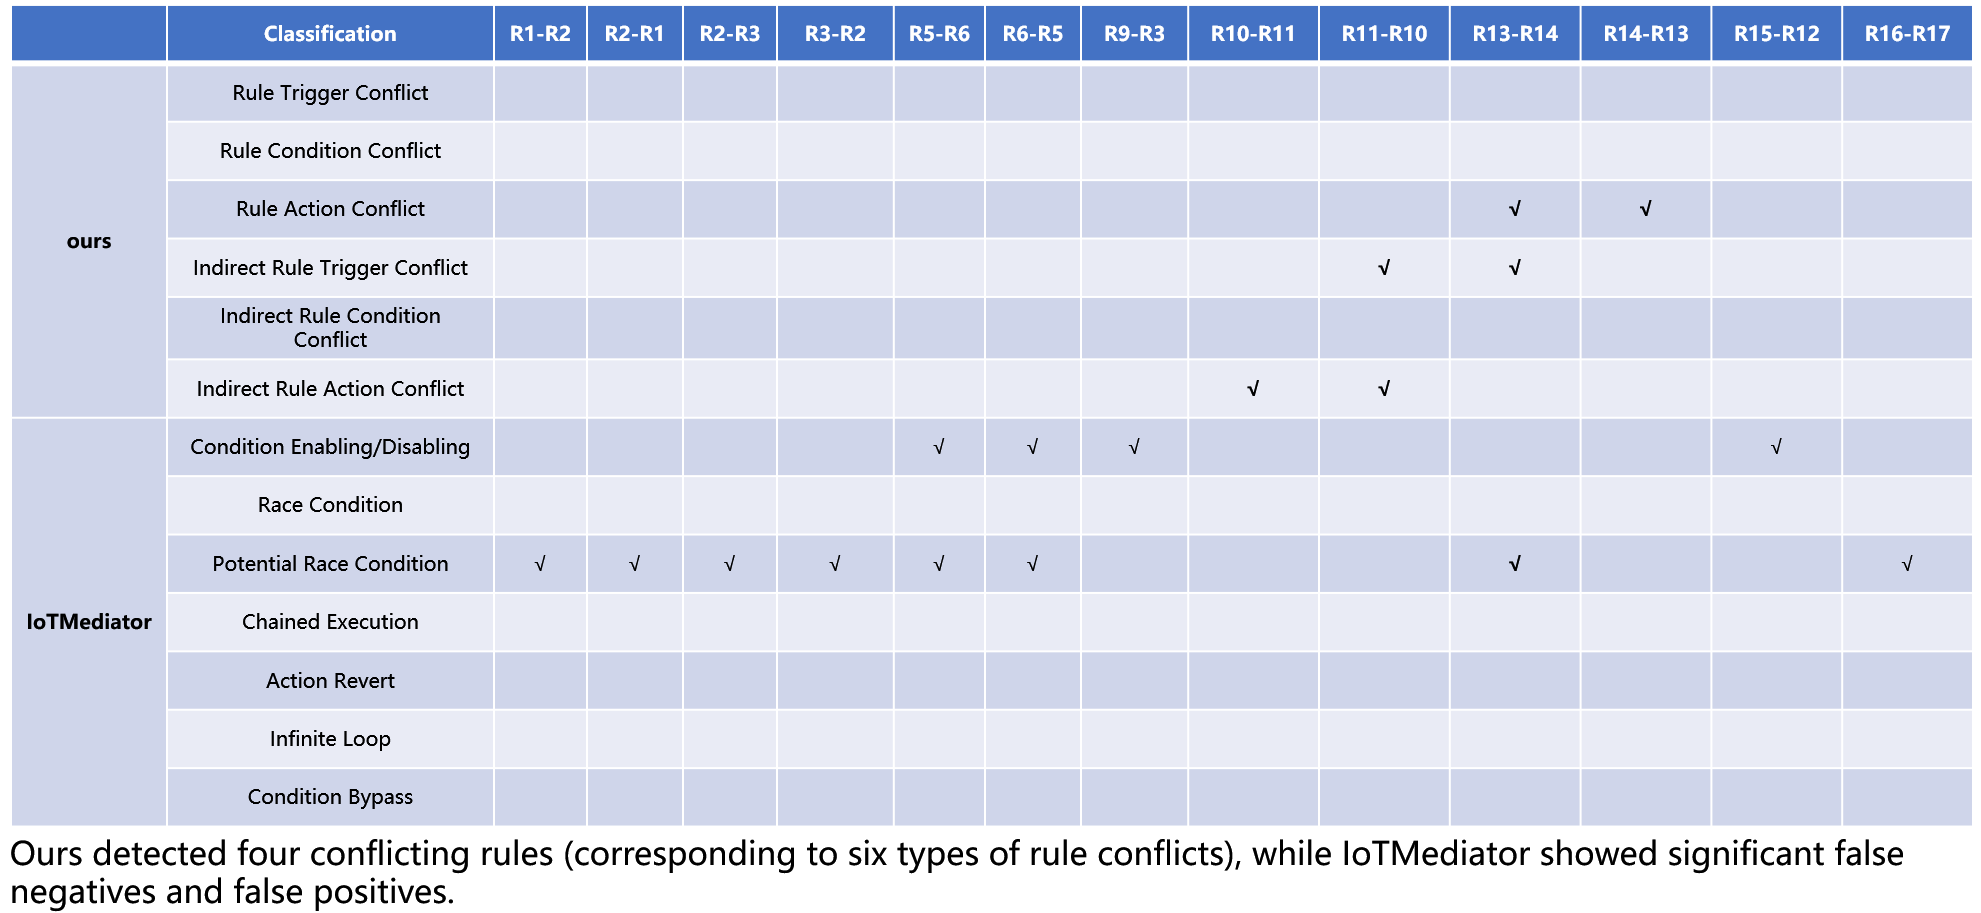
\includegraphics[width=\textwidth]{figure/conflict_detection_result.png}
	\caption{Result of Rule Conflict Detection}
	\label{conflict_detection_result}
\end{figure*}

\subsection{Effectiveness of Conflict Resolution}

\begin{figure}[htbp]
	\centering
	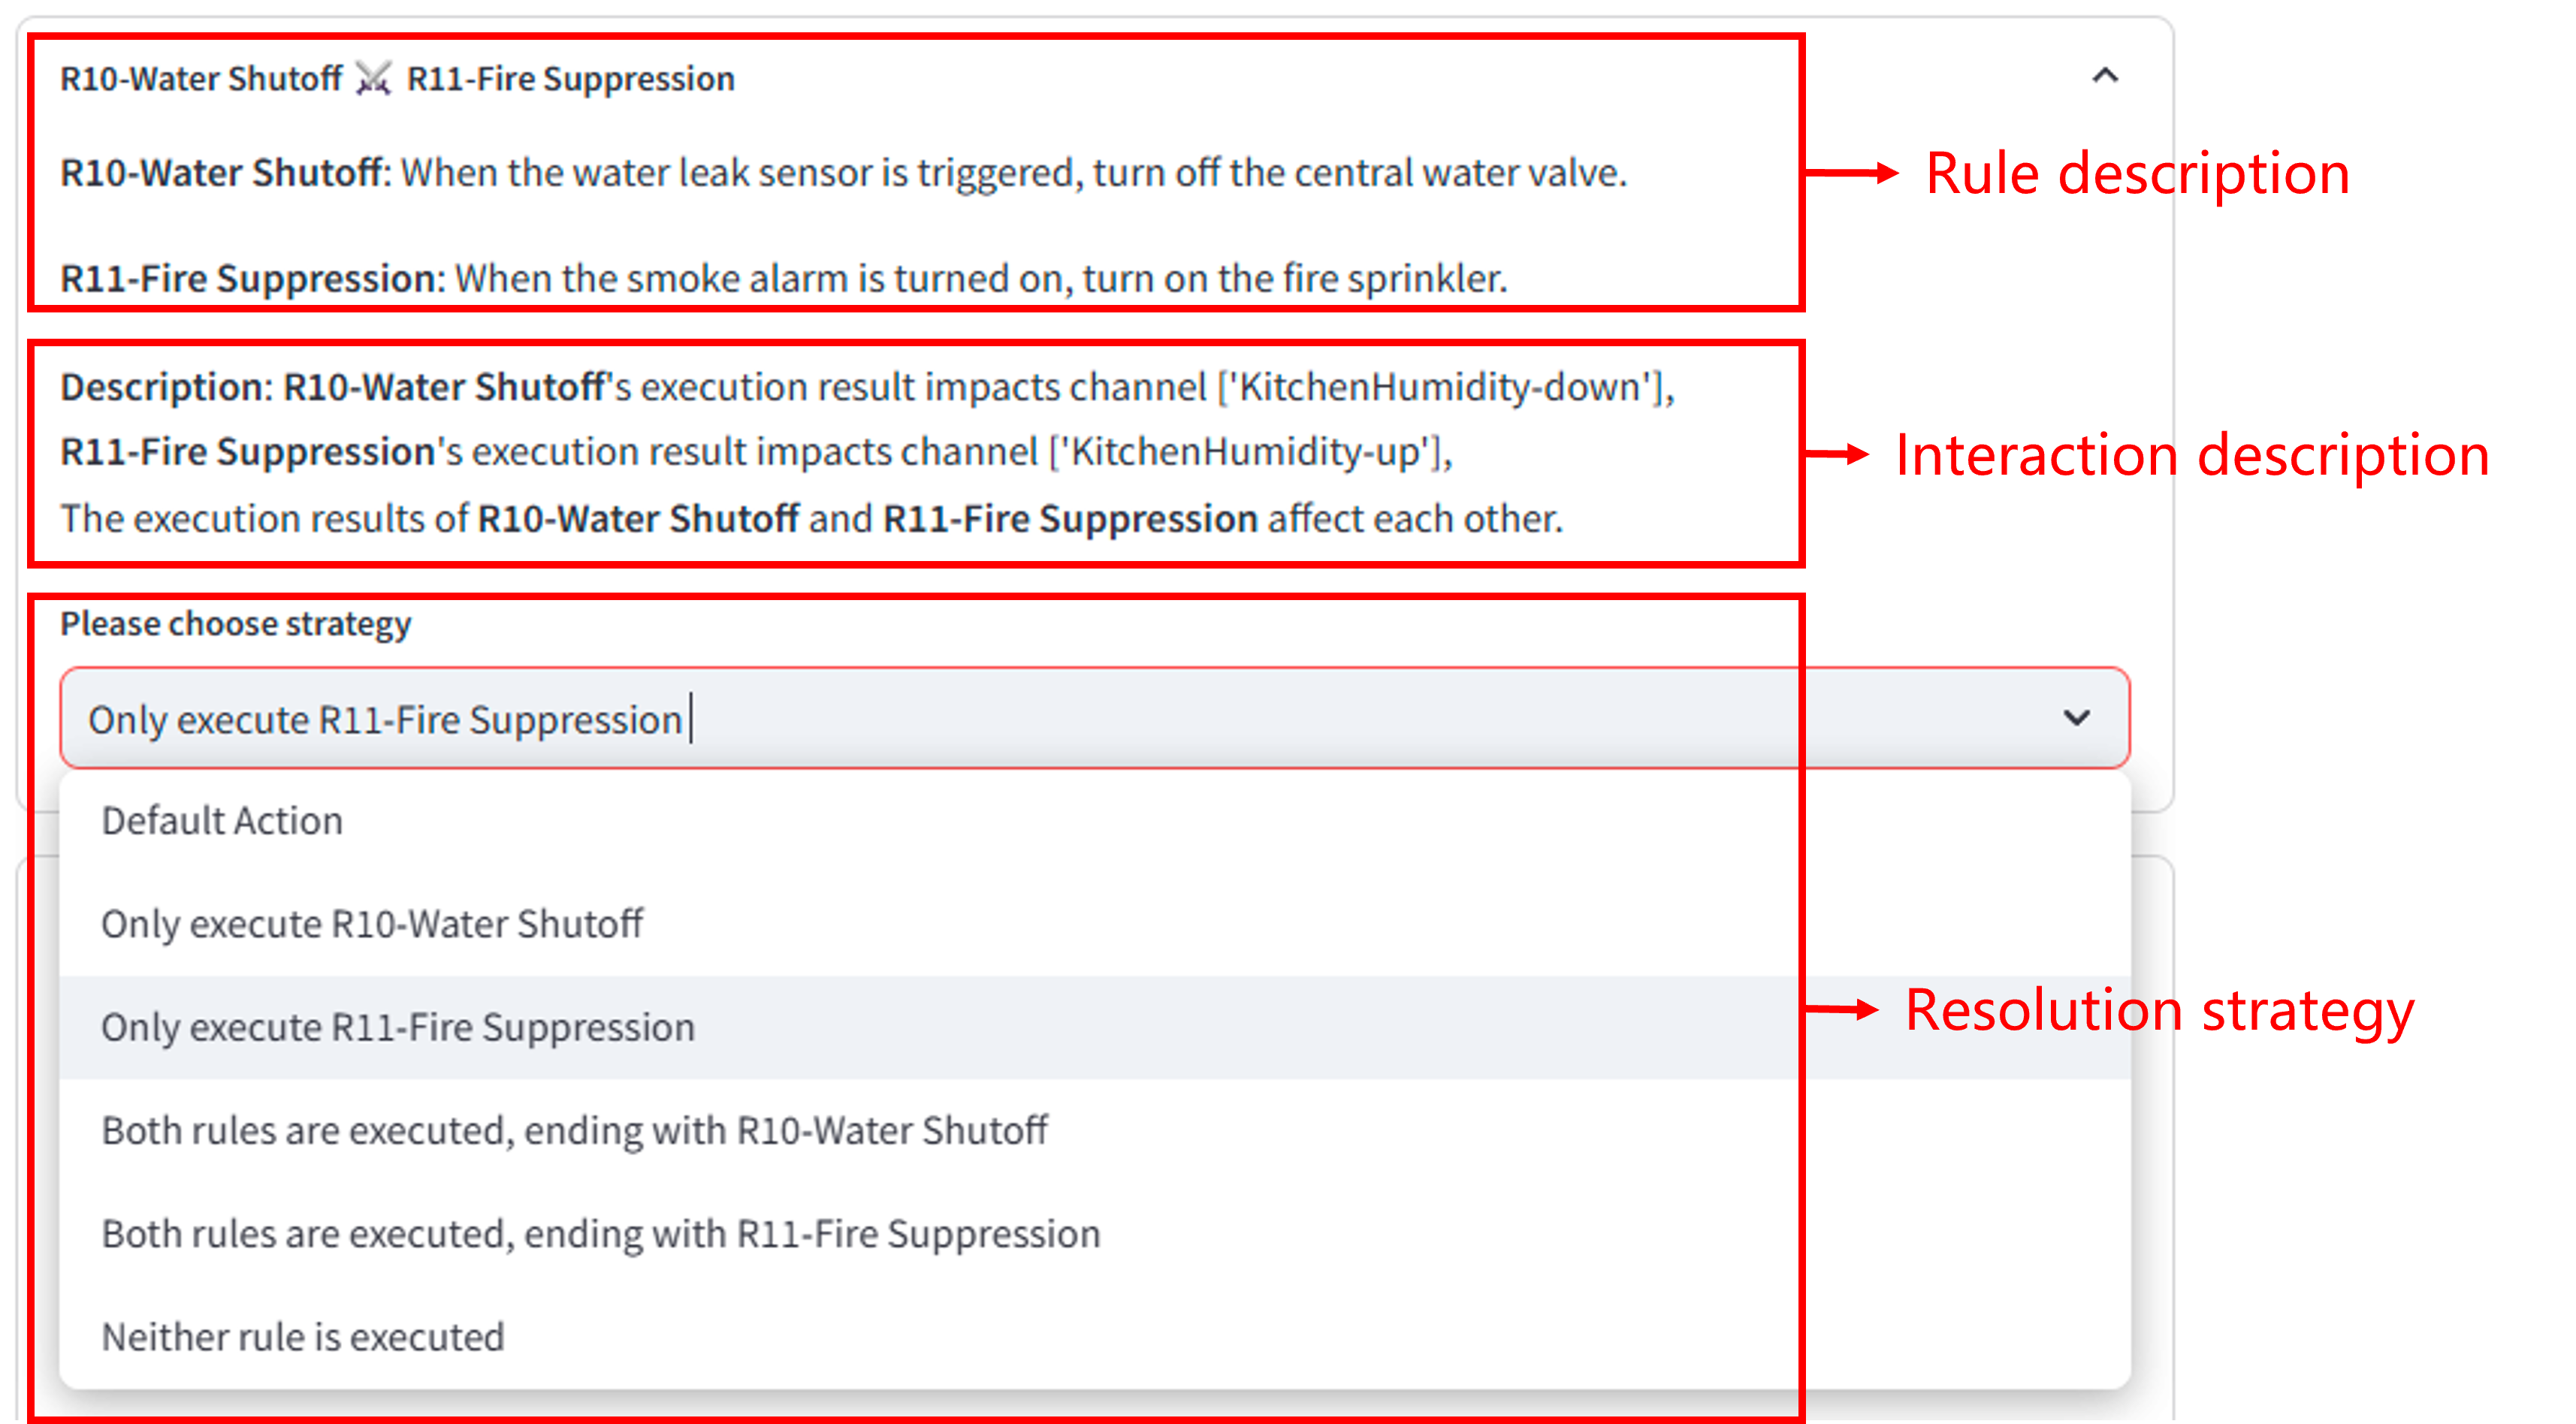
\includegraphics[width=0.45\textwidth]{figure/resolution_example.png}
	\caption{Example of Automated Rule Conflict Resolution}
	\label{example_resolution}
\end{figure}

%为了评估自动化的规则冲突处理的可用性,本章节将结合具体的示例展示对于一个具体的规则冲突,系统如何进行自动化处理,以及AI对于系统提供的规则冲突信息的推测处理方式。
In order to assess the effectiveness of automated rule conflict resolution, this chapter will use specific examples to demonstrate how the system automatically processes a particular rule conflict and how AI speculatively handles the rule conflict information provided by the system.

%Fig.\ref{example_resolution}展示了规则R10与规则R11对应的Indirect Action Conflict。图片中展示了规则的描述(自动化规则配置文件中提取得到),规则冲突描述(Rule Conflict Detection Module中根据上下文信息生成)为:R10-Water Shutoff's execution result impacts channel ['KitchenHumidity-down'],R11-Fire Suppression's execution result impacts channel ['KitchenHumidity-up'],The execution results of R10-Water Shutoff and R11-Fire Suppression affect each other.最下面是处理策略,包含一个默认执行动作和五个规则冲突缓解动作。
Fig.\ref{example_resolution} displays the Indirect Action Conflict corresponding to rules R10 and R. The image shows the description of the rules (extracted from the automated rule configuration file) and the rule conflict description (generated by the Rule Conflict Detection Module based on contextual information) as: R10-Water Shutoff's execution result impacts channel ['KitchenHumidity-down'], R11-Fire Suppression's execution result impacts channel ['KitchenHumidity-up'], and the execution results of R10-Water Shutoff and R11-Fire Suppression affect each other. At the bottom is the resolution strategy, which consists of a default execution action and five rule conflict mitigation actions.

%根据实体安全配置,规则R10的执行动作将水阀关闭,使用线性函数进行评估,其对应的安全值参数$sf_{R10}=-1$,而R11的执行动作将开启消防喷淋头,其对应的安全值参数$sf_{R11}=1$,因此Generation of Resolution Strategy Module将会自动化推荐“Only excute R11”策略用于预防规则冲突的真实发生。除此之外页面的对处理策略提供选项,用户可以对规则冲突处理策略进行选择,以选择更符合偏好的处理方案。
According to the entity security configuration, the execution action of rule R10 will close the water valve, and its evaluation is conducted using a linear function with the corresponding safety parameter $sf_{R10}=-1$, while the execution action of rule R11 will activate the fire sprinkler head, with its corresponding safety parameter $sf_{R11}=1$. Therefore, the Generation of Resolution Strategy Module will automatically recommend the "Only execute R11" strategy to prevent real conflicts between rules. In addition, the page provides options for resolution strategies, allowing users to choose a rule conflict resolution strategy that better fits their preferences.

%为了测试Rule Conflict Detection Module根据规则模型生成的规则冲突描述对用户的友好性,本论文使用AI测试其对规则冲突的处理策略选择。仍旧以Fig.\ref{example_resolution}为例,使用的模型为gpt-4o-2024-11-20,调用方式为OPENAI API,其它参数默认不做修改,系统提示词将会展示在 Appendix.\ref{apdx:system_prompt}。对于上述示例我们得到的回复如下:\texttt{\{
%		"policy": "2", // Only execute R11
%		"reason": "In this case of Indirect Rule Action Conflict, the sprinkler system activated by R11 is crucial for safety during a fire, and its priority should supersede the water cutoff triggered by R10 to ensure effective fire suppression. Therefore, only R11 should execute."
%	\}}
To test the user-friendliness of the rule conflict description generated according to the rule model by the Rule Conflict Detection Module, we uses AI to test its strategy selection for conflict resolution. Still taking Fig.\ref{example_resolution} as an example, the model used is \texttt{gpt-4o-2024-11-20}, called via the OPENAI API, with other parameters remaining unchanged by default, and the system prompt will be shown in Appendix.\ref{apdx:system_prompt}. For the above example, we obtained the following response: 
\texttt{\{\\
	"policy": "2", // Only execute R11 \\
	"reason": "In this case of Indirect Rule Action Conflict, the sprinkler system activated by R11 is crucial for safety during a fire, and its priority should supersede the water cutoff triggered by R10 to ensure effective fire suppression. Therefore, only R11 should execute."\\
	\}}\\

%通过AI对规则冲突描述的理解对规则冲突处理策略的推荐结果与预期相契合,一定程度上标明当前的提取的规则冲突信息能够很好地被用户理解,并作出正确有效的选择,也为用户提供了使用智能工具进行规则冲突处理策略推荐的选择。
Through AI's understanding of rule conflict descriptions, the recommended results for rule conflict resolution strategies align with expectations, which to some extent indicates that the currently extracted rule conflict information can be well understood by users, enabling them to make correct and effective choices, and providing them with the option to use intelligent tools for recommending rule conflict resolution strategies.

\subsection{Performance} 
%为了测试系统性能,本论文根据系统架构将测试分为静态分析的性能评估与动态检测与冲突处理的性能评估。
In order to test the system performance, we divides the testing into performance evaluation of static analysis and performance evaluation of dynamic detection and conflict based on the system architecture.

%其中静态检测的性能评估中,静态检测会遍历所有的自动化规则(包含Formal Analysis Module和Rule Conflict Detection Module),并对每两种规则进行比较,还将进行自比较,因此对于n条规则来说,静态检测的时间复杂度为$O\left(n^2\right)$。对于测试使用AI生成的100条规则集(100条)与1000条规则集(1000条)作为输入评估多次检测耗时,单位为秒,为便于展示选择其中三次检测结果并记录平均值,Table.\ref{performance_static_analysis}展示了测试的结果。可以观察到即使存在1000条规则,静态检测也只需要约$12s$,不同数据量的静态检测耗时符合预期的复杂度。
In the performance evaluation of static detection, static detection traverses all automation rules (including the Formal Analysis Module and Rule Conflict Detection Module) and compares every two rules, as well as performing self-comparison. Therefore, for n rules, the time complexity of static detection is $O\left(n^2\right)$. For testing, an AI-generated set of 100 rules (100 rules) and a set of 1000 rules (1000 rules) were used as inputs to evaluate the detection time multiple times, in seconds. To facilitate the display, three detection results were selected and the average value was recorded. Table.\ref{performance_static_analysis} shows the test results. It can be observed that even with 1000 rules, static detection only takes about $12s$, and the static detection time for different data volumes meets the expected complexity.

\begin{figure}[htbp]
	\caption{Performance of Static Analysis}
	\label{performance_static_analysis}
	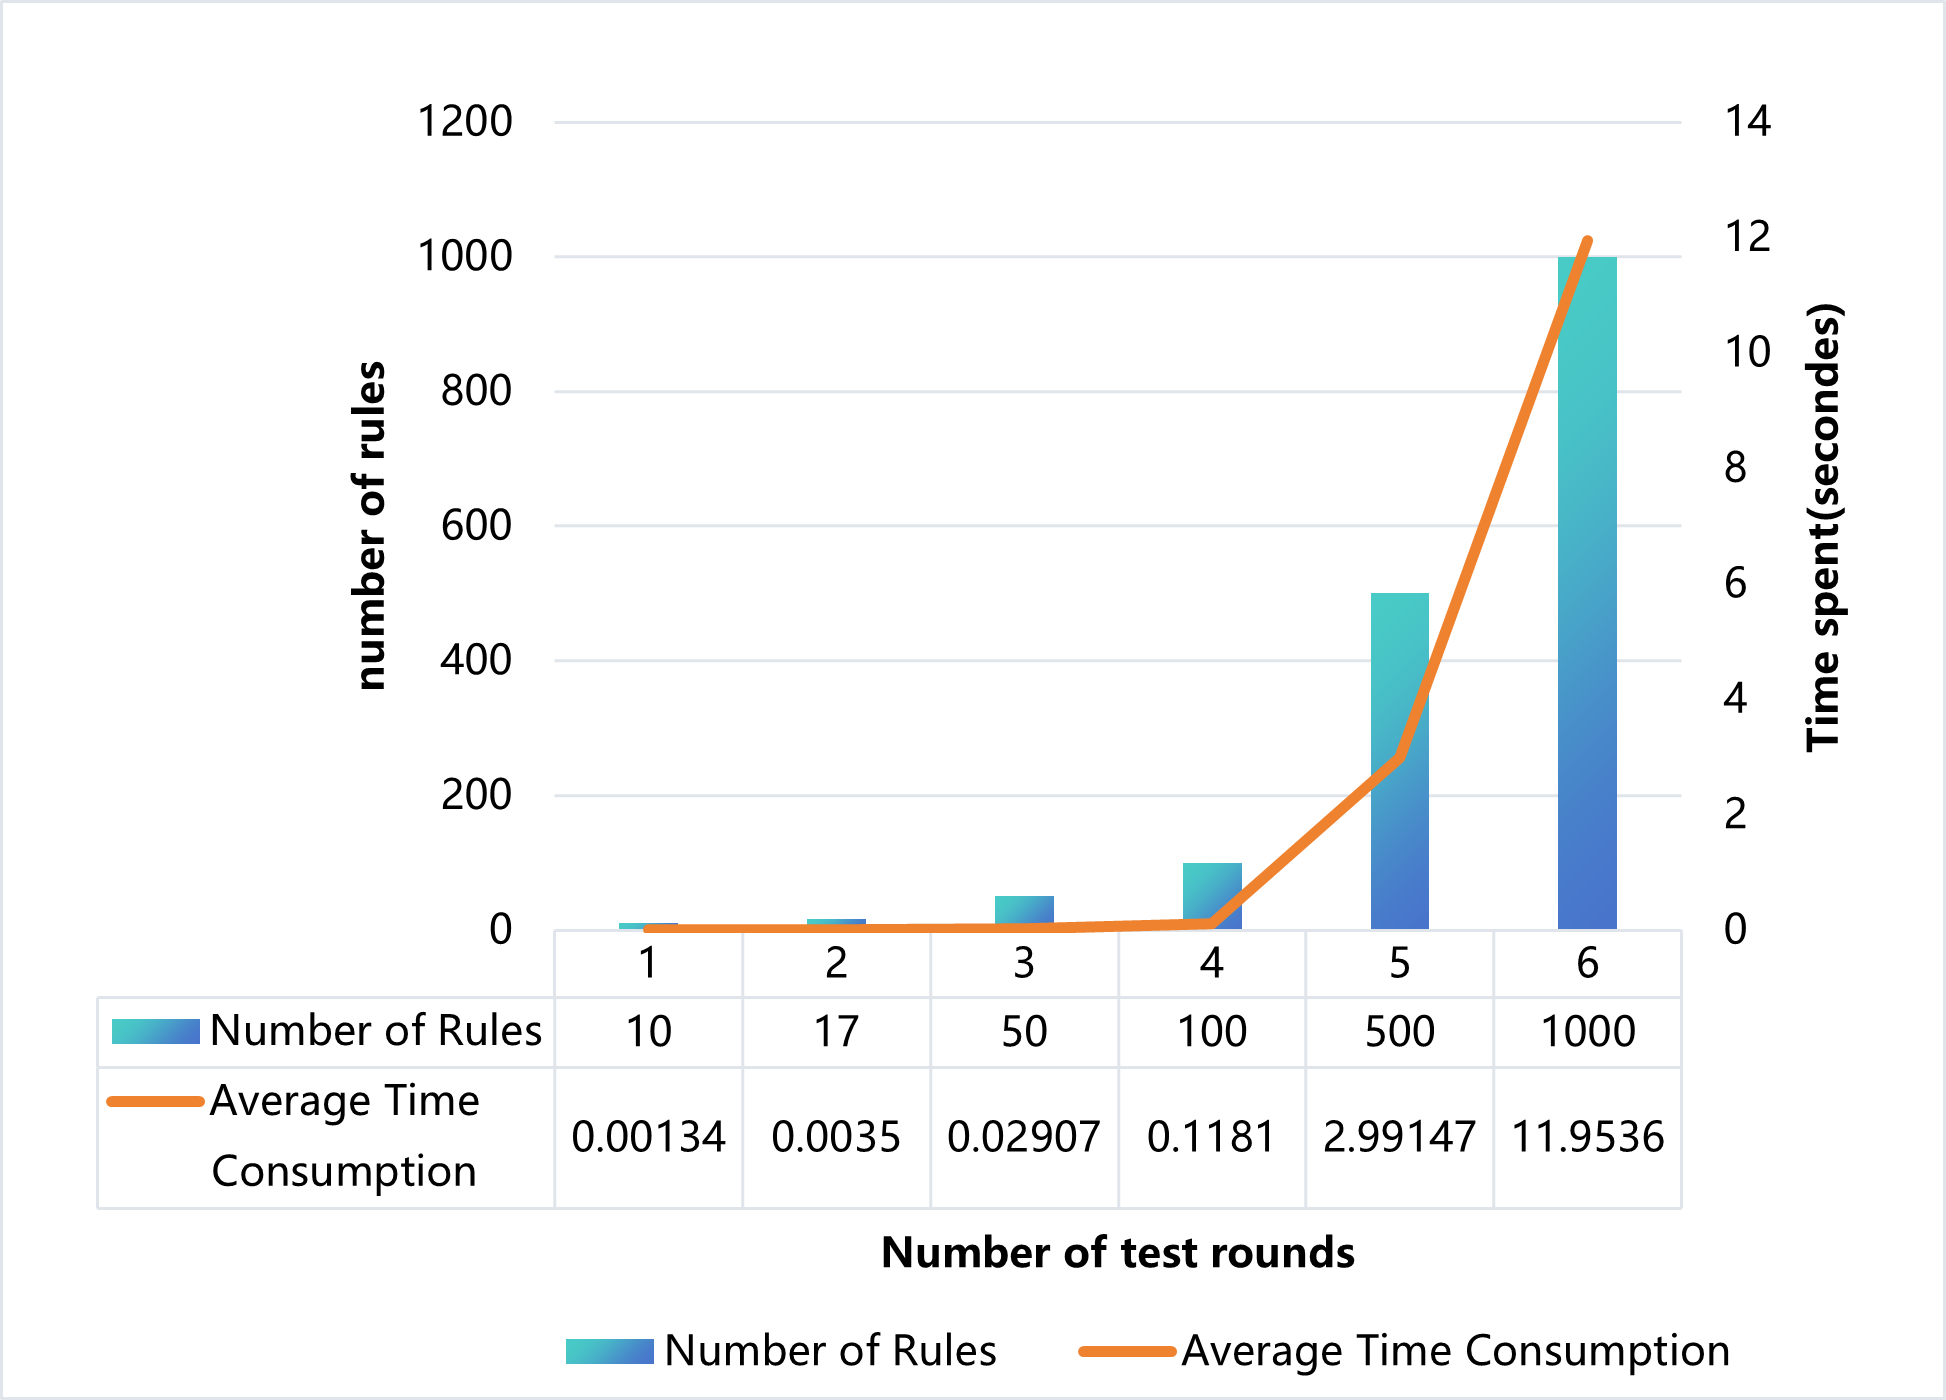
\includegraphics[width=0.5\textwidth]{figure/performance.png}
	
\end{figure}

%在规则冲突动态检测(Assertion Verification Module)与规则冲突处理指令生成(Command Generation Module)两个模块中,其本身计算量不高,时间消耗主要体现在通信过程,因此接下来着重进行代码插桩装通信性能评估,测试包括随机触发规则冲突,对所有通信函数(包括系统发送消息,Home Assistant平台处理完毕返回消息,系统接收到消息三个阶段)的性能测评,通信函数的介绍与性能测评结果如Table.\ref{performance_communication_function}所示。
In the two modules—the Assertion Detection Module for detecting rule conflicts dynamically and the Command Generation Module for handling rule conflict processing—the computational load is not high, and the time consumption mainly lies in the communication process. Therefore, the focus will next be on code instrumentation for communication performance evaluation, testing which includes randomly triggering rule conflicts and assessing the performance of all communication functions (covering the three stages of system sending messages, Home Assistant platform processing and returning messages, and system receiving messages). The introduction and performance evaluation results of the communication functions are shown in Table.\ref{performance_communication_function}.

%可以观察到在实验环境中的通信函数平均与最长耗时仅有毫秒级别,且在断言验证与规则冲突处理方案指令生成两个步骤中只会调用有限次数的通信函数,且耗时均也只有毫秒级别。
It can be observed that the average and maximum time consumption of the communication functions in the experimental environment are only at the millisecond level, and that only a limited number of calls are made to the communication functions during the two steps of assertion verification and rule conflict handling directive generation, with each call also taking only a few milliseconds.

\begin{table*}[htpb]
	\caption{Performance of Communication Functions}
	\label{performance_communication_function}
	\centering
	\begin{adjustbox}{width=0.95\textwidth}
		\begin{tabular}{c|c|c|c}
			\hline
			\textbf{Function Name} & \textbf{Description} & \textbf{Average Time Consumption} & \textbf{Maximum Time Consumption}\\
			\hline
			get\_entity\_state & Get entity state & $1.193 \times 10^{-3}$s & $1.953 \times 10^{-3}$s \\
			\hline
			time\_now & Get HomeAssistant system time & $9.765 \times 10^{-4}$s & $9.825 \times 10^{-4}$s \\
			\hline
			command\_send & Send conflict handling command & $9.643 \times 10^{-4}$s & $9.787 \times 10^{-4}$s \\
			\hline
			communicate\_finish & End communication phase & $9.778 \times 10^{-4}$s & $9.832 \times 10^{-4}$s \\
			\hline
			\multicolumn{4}{l}{Note: Each function is tested 10 times.} \\
		\end{tabular}
	\end{adjustbox}
\end{table*}